\section{Auswertung}
\label{sec:Auswertung}
\subsection{Bestimmung der maximalen Feldstärke}
Um die maximale Feldstärke zu bestimmen, wird eine Hallsonde entlang der $z$-Achse verschoben und die damit gemessene 
Feldstärke wird notiert.
Die Messwerte sind in Tabelle \ref{tab:Feldstärke} aufgelistet.
\FloatBarrier
\begin{table}
  \centering
  \begin{tabular}{c c}
    \toprule
    $z$ / \SI{}{\milli\meter}& $B$ / \SI{}{\milli\tesla}\\
    \midrule
    125& 202\\     
    123& 298\\
    121& 359\\
    119& 389\\
    117& 404\\
    116& 406\\
    115& 410\\
    114& 409\\
    113& 409\\
    111& 402\\
    109& 386\\
    107& 355\\
    \bottomrule
  \end{tabular}
  \caption{Messwerte zur Bestimmung der maximalen Feldstärke.}
  \label{tab:Feldstärke}
\end{table}
\FloatBarrier
Die Werte aus der Tabelle \ref{tab:Feldstärke} werden in Abbildung \ref{fig:Feldstärke} dargestellt.
\FloatBarrier
\begin{figure}
  \centering
  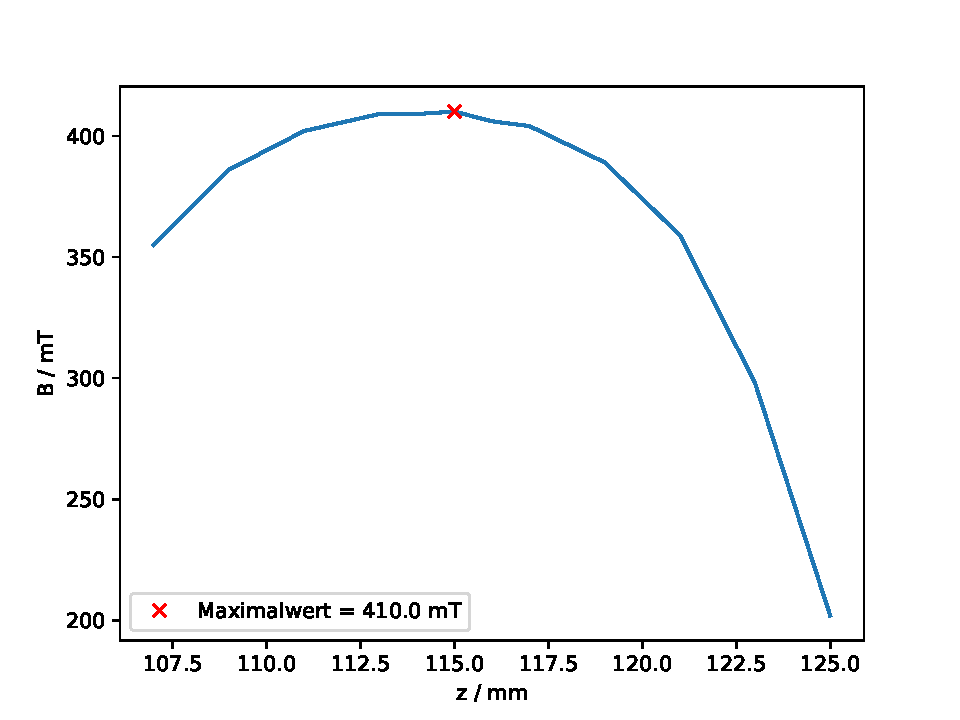
\includegraphics[width = \textwidth, keepaspectratio]{figure/BFeld_plot.pdf}
  \caption{Graphische Darstellung der Messwerte für die Bestimmung der maximalen Feldstärke}
  \label{fig:Feldstärke}
\end{figure}
\FloatBarrier
Der Maximale Wert liegt bei $\SI{410}{\milli\tesla}$. 
\subsection{Bestimmung der effektiven Masse}
Für die Bestimmung der effektiven Masse wird der Drehwinkel der Polarisationsebene in Abhängigkeit der Wellenlänge gemessen.
Diese Daten werden für zwei n-dotierte und eine reine Probe aufgenommen. Da die Proben unterschiedlich dick sind, wird 
der Drehwinkel auf die Dicke der Probe normiert.
Der Drehwinkel wird bestimmt, indem zwei Winkel gemessen werden, bei betragsmäßig gleichem Magnetfeld, allerdings
um $\SI{180}{\degree}$ gedreht. Aus diesen beiden Winkeln lässt sich der eigentliche Drehwinkel über die Formel
\begin{equation*}
  \theta=\frac{\theta_1 - \theta_2}{2}
\end{equation*}
Die Messwerte sind in den Tabellen \ref{tab:Drehwinkel_1} - \ref{tab:Drehwinkel_3} notiert, in Tabelle \ref{tab:Drehwinkel_norm} sind die normierten Drehwinkel aufgelistet.
\FloatBarrier
\begin{table}
  \centering
  \begin{tabular}{c c c c}
    \toprule
    $\lambda$ / \SI{}{\micro\meter}&$\theta_1$ / $\SI{}{\degree}$&$\theta_2$ / $\SI{}{\degree}$&$\theta$ / $\SI{}{\degree}$ \\
    \midrule
    $\num{1.06} $&$\num{214.52}$&$\num{184.53}$&$\num{14.99}$\\
    $\num{1.29} $&$\num{209.33}$&$\num{193.58}$&$\num{7.88}$\\
    $\num{1.45} $&$\num{151.18}$&$\num{148.0}$&$\num{1.59}$\\
    $\num{1.72} $&$\num{152.92}$&$\num{149.67}$&$\num{1.62}$\\
    $\num{1.96} $&$\num{157.17}$&$\num{147.25}$&$\num{4.96}$\\
    $\num{2.156}$&$\num{158.52}$&$\num{151.07}$&$\num{3.73}$\\
    $\num{2.34} $&$\num{188.72}$&$\num{175.92}$&$\num{6.4}$\\
    $\num{2.51} $&$\num{218.0}$&$\num{190.45}$&$\num{13.78}$\\
    $\num{2.65} $&$\num{164.1}$&$\num{155.58}$&$\num{4.26}$\\
    \bottomrule
  \end{tabular}
  \caption{Drehwinkel der Probe 1 mit der Dicke $d=\SI{1360}{\micro\meter}$, in Abhängigkeit der Wellenlänge.}
  \label{tab:Drehwinkel_1}
\end{table}

\begin{table}
  \centering
  \begin{tabular}{c c c c}
    \toprule
    $\lambda$ / \SI{}{\micro\meter}&$\theta_1$ / $\SI{}{\degree}$&$\theta_2$ / $\SI{}{\degree}$&$\theta$ / $\SI{}{\degree}$ \\
    \midrule
    $\num{1.06} $&$\num{155.53}$&$\num{143.87}$&$\num{5.83}$\\
    $\num{1.29} $&$\num{154.32}$&$\num{145.0}$&$\num{4.66}$\\
    $\num{1.45} $&$\num{153.23}$&$\num{144.18}$&$\num{4.52}$\\
    $\num{1.72} $&$\num{155.1}$&$\num{145.4}$&$\num{4.85}$\\
    $\num{1.96} $&$\num{160.0}$&$\num{149.23}$&$\num{5.38}$\\
    $\num{2.156}$&$\num{161.15}$&$\num{149.08}$&$\num{6.03}$\\
    $\num{2.34} $&$\num{186.45}$&$\num{173.43}$&$\num{6.51}$\\
    $\num{2.51} $&$\num{207.07}$&$\num{191.82}$&$\num{17.62}$\\
    $\num{2.65} $&$\num{165.63}$&$\num{152.0}$&$\num{6.82}$\\
    \bottomrule
  \end{tabular}
  \caption{Drehwinkel der Probe 2 mit der Dicke $d=\SI{1296}{\micro\meter}$, in Abhängigkeit der Wellenlänge.}
  \label{tab:Drehwinkel_2}
\end{table}

\begin{table}
  \centering
  \begin{tabular}{c c c c}
    \toprule
    $\lambda$ / \SI{}{\micro\meter}&$\theta_1$ / $\SI{}{\degree}$&$\theta_2$ / $\SI{}{\degree}$&$\theta$ / $\SI{}{\degree}$ \\
    \midrule
    $\num{1.06} $&$\num{161.47}$&$\num{138.07}$&$\num{11.7}$\\
    $\num{1.29} $&$\num{158.87}$&$\num{141.45}$&$\num{8.71}$\\
    $\num{1.45} $&$\num{155.05}$&$\num{142.0}$&$\num{6.53}$\\
    $\num{1.72} $&$\num{154.8}$&$\num{144.77}$&$\num{5.02}$\\
    $\num{1.96} $&$\num{157.45}$&$\num{150.5}$&$\num{3.47}$\\
    $\num{2.156}$&$\num{157.12}$&$\num{151.68}$&$\num{2.72}$\\
    $\num{2.34} $&$\num{182.53}$&$\num{177.57}$&$\num{2.48}$\\
    $\num{2.51} $&$\num{34.78}$&$\num{31.2}$&$\num{1.79}$\\
    $\num{2.65} $&$\num{163.55}$&$\num{158.02}$&$\num{2.77}$\\
    \bottomrule
  \end{tabular}
  \caption{Drehwinkel der reinen Probe mit der Dicke $d=\SI{5110}{\micro\meter}$, in Abhängigkeit der Wellenlänge.}
  \label{tab:Drehwinkel_3}
\end{table}

\begin{table}
  \centering
  \begin{tabular}{c c c c}
    \toprule
    $\lambda$ / \SI{}{\micro\meter}& $\theta_{\text{n-dotiert 1}}$ / $\frac{\SI{}{\radian}}{\SI{}{\micro\meter}}$& 
    $\theta_{\text{n-dotiert 2}}$ / $\frac{\SI{}{\radian}}{\SI{}{\micro\meter}}$&
    $\theta_{\text{rein}}$ / $\frac{\SI{}{\radian}}{\SI{}{\micro\meter}}$\\
    \midrule
    $\num{1.06} $&$\num{1.92e-4}$&$\num{0.79e-4}$&$\num{0.4e-4}$\\
    $\num{1.29} $&$\num{1.01e-4}$&$\num{0.63e-4}$&$\num{0.3e-4}$\\
    $\num{1.45} $&$\num{0.2e-4}$&$\num{0.61e-4}$&$\num{0.22e-4}$\\
    $\num{1.72} $&$\num{0.21e-4}$&$\num{0.65e-4}$&$\num{0.17e-4}$\\
    $\num{1.96} $&$\num{0.64e-4}$&$\num{0.72e-4}$&$\num{0.12e-4}$\\
    $\num{2.156}$&$\num{0.48e-4}$&$\num{0.81e-4}$&$\num{0.09e-4}$\\
    $\num{2.34} $&$\num{0.82e-4}$&$\num{0.88e-4}$&$\num{0.08e-4}$\\
    $\num{2.51} $&$\num{1.77e-4}$&$\num{1.03e-4}$&$\num{0.06e-4}$\\
    $\num{2.65} $&$\num{0.55e-4}$&$\num{0.92e-4}$&$\num{0.09e-4}$\\
    \bottomrule
  \end{tabular}
  \caption{Normierter Drehwinkel in Abhängigkeit der Wellenlänge. Die Dicken der Probe sind: Probe 1 $d=\SI{1360}{\micro\meter}$,
  Probe 2 $d=\SI{1296}{\micro\meter}$, reine Probe $d=\SI{5110}{\micro\meter}$.}
  \label{tab:Drehwinkel_norm}
\end{table}
\FloatBarrier
Die Daten aus Tabelle \ref{tab:Drehwinkel_norm} werden in Abbildung \ref{fig:Drehwinkel_1} und \ref{fig:Drehwinkel_2} 
dargestellt.
\FloatBarrier
\begin{figure}
  \centering
  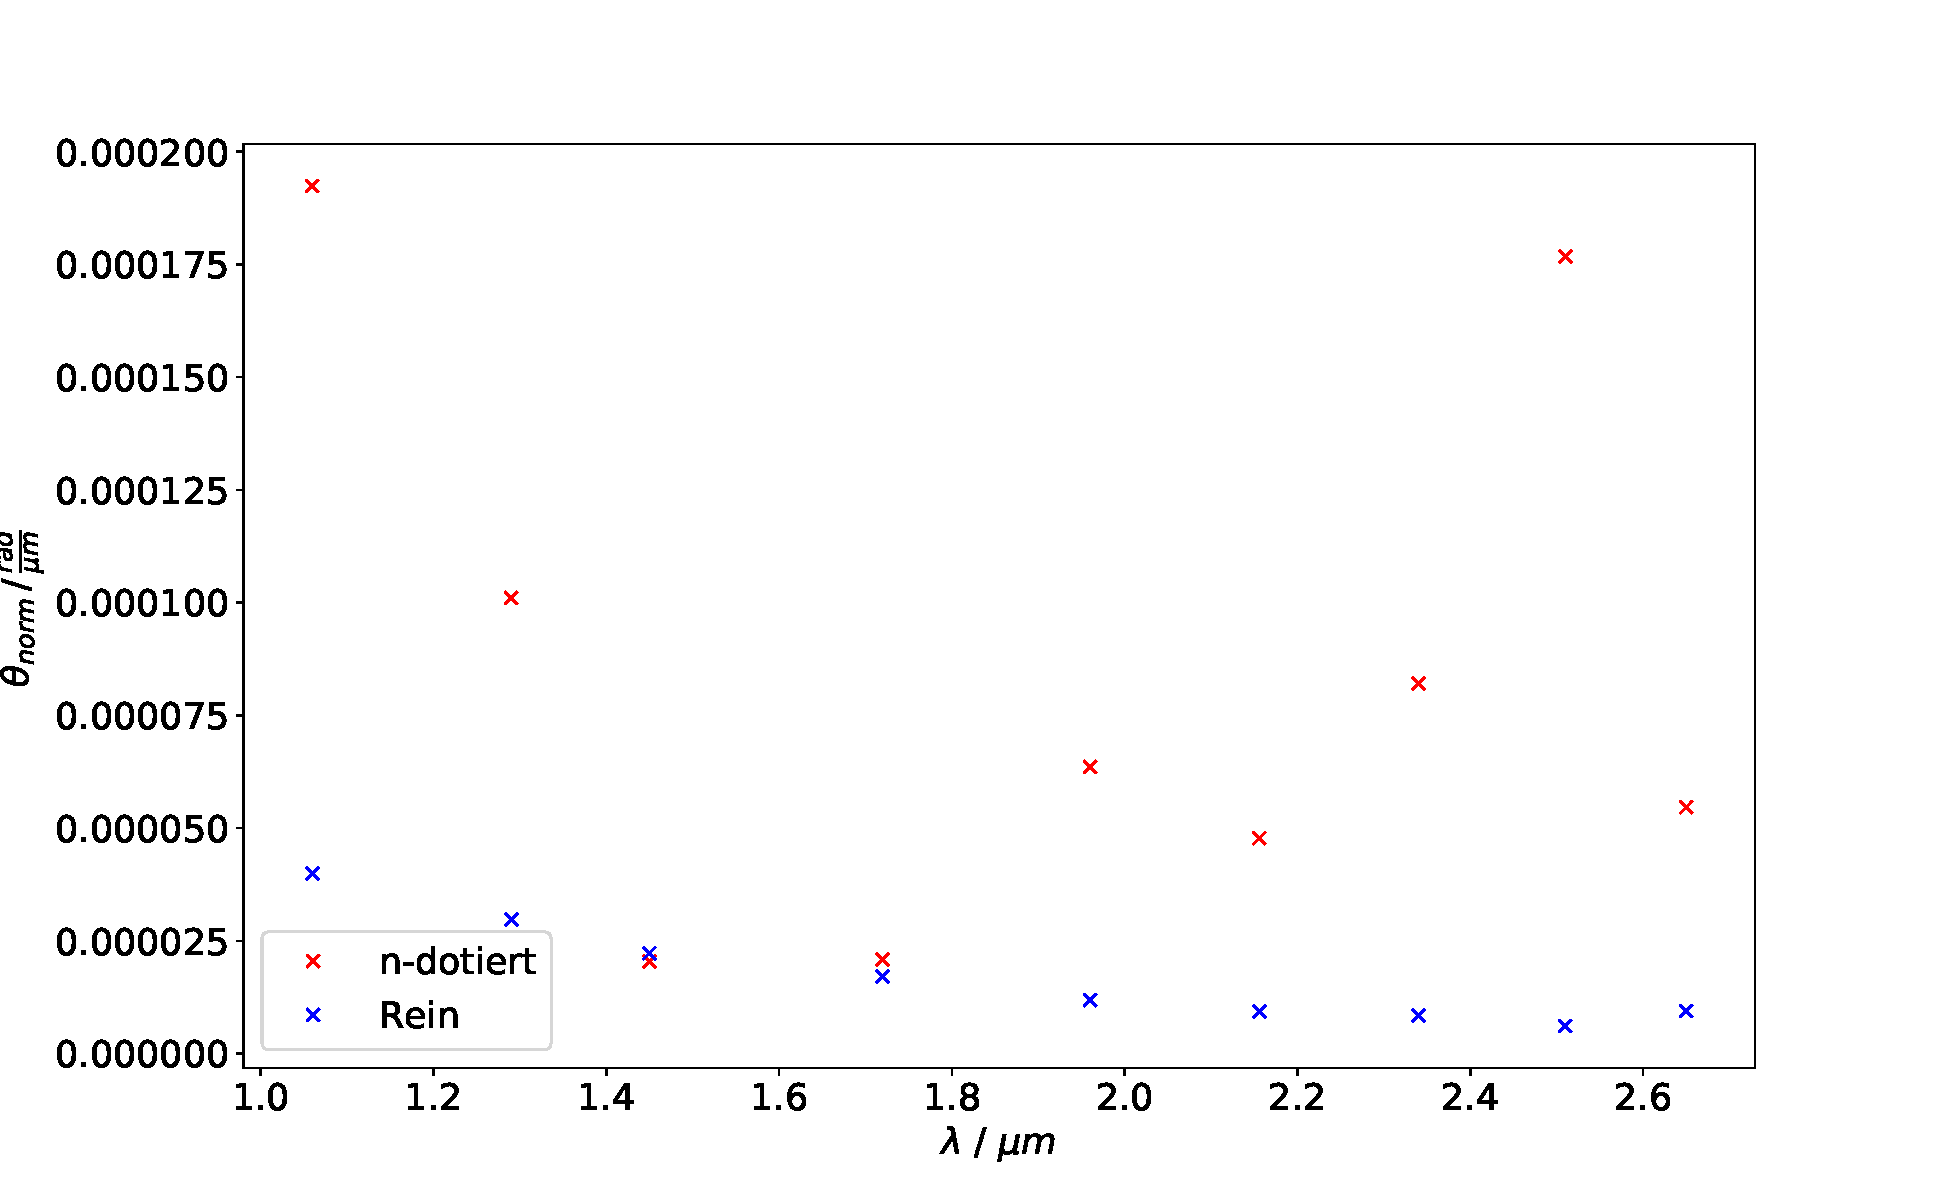
\includegraphics[width = \textwidth,keepaspectratio]{figure/Theta1_plot.pdf}
  \caption{Graphische Darstellung der normierten Drehwinkel, in Abhängigkeit der Wellenlänge, von der Probe 1 mit einer Dicke von $d=\SI{1360}{\micro\meter}$ und 
  der reinen Probe.}
  \label{fig:Drehwinkel_1}
\end{figure}
\begin{figure}
  \centering
  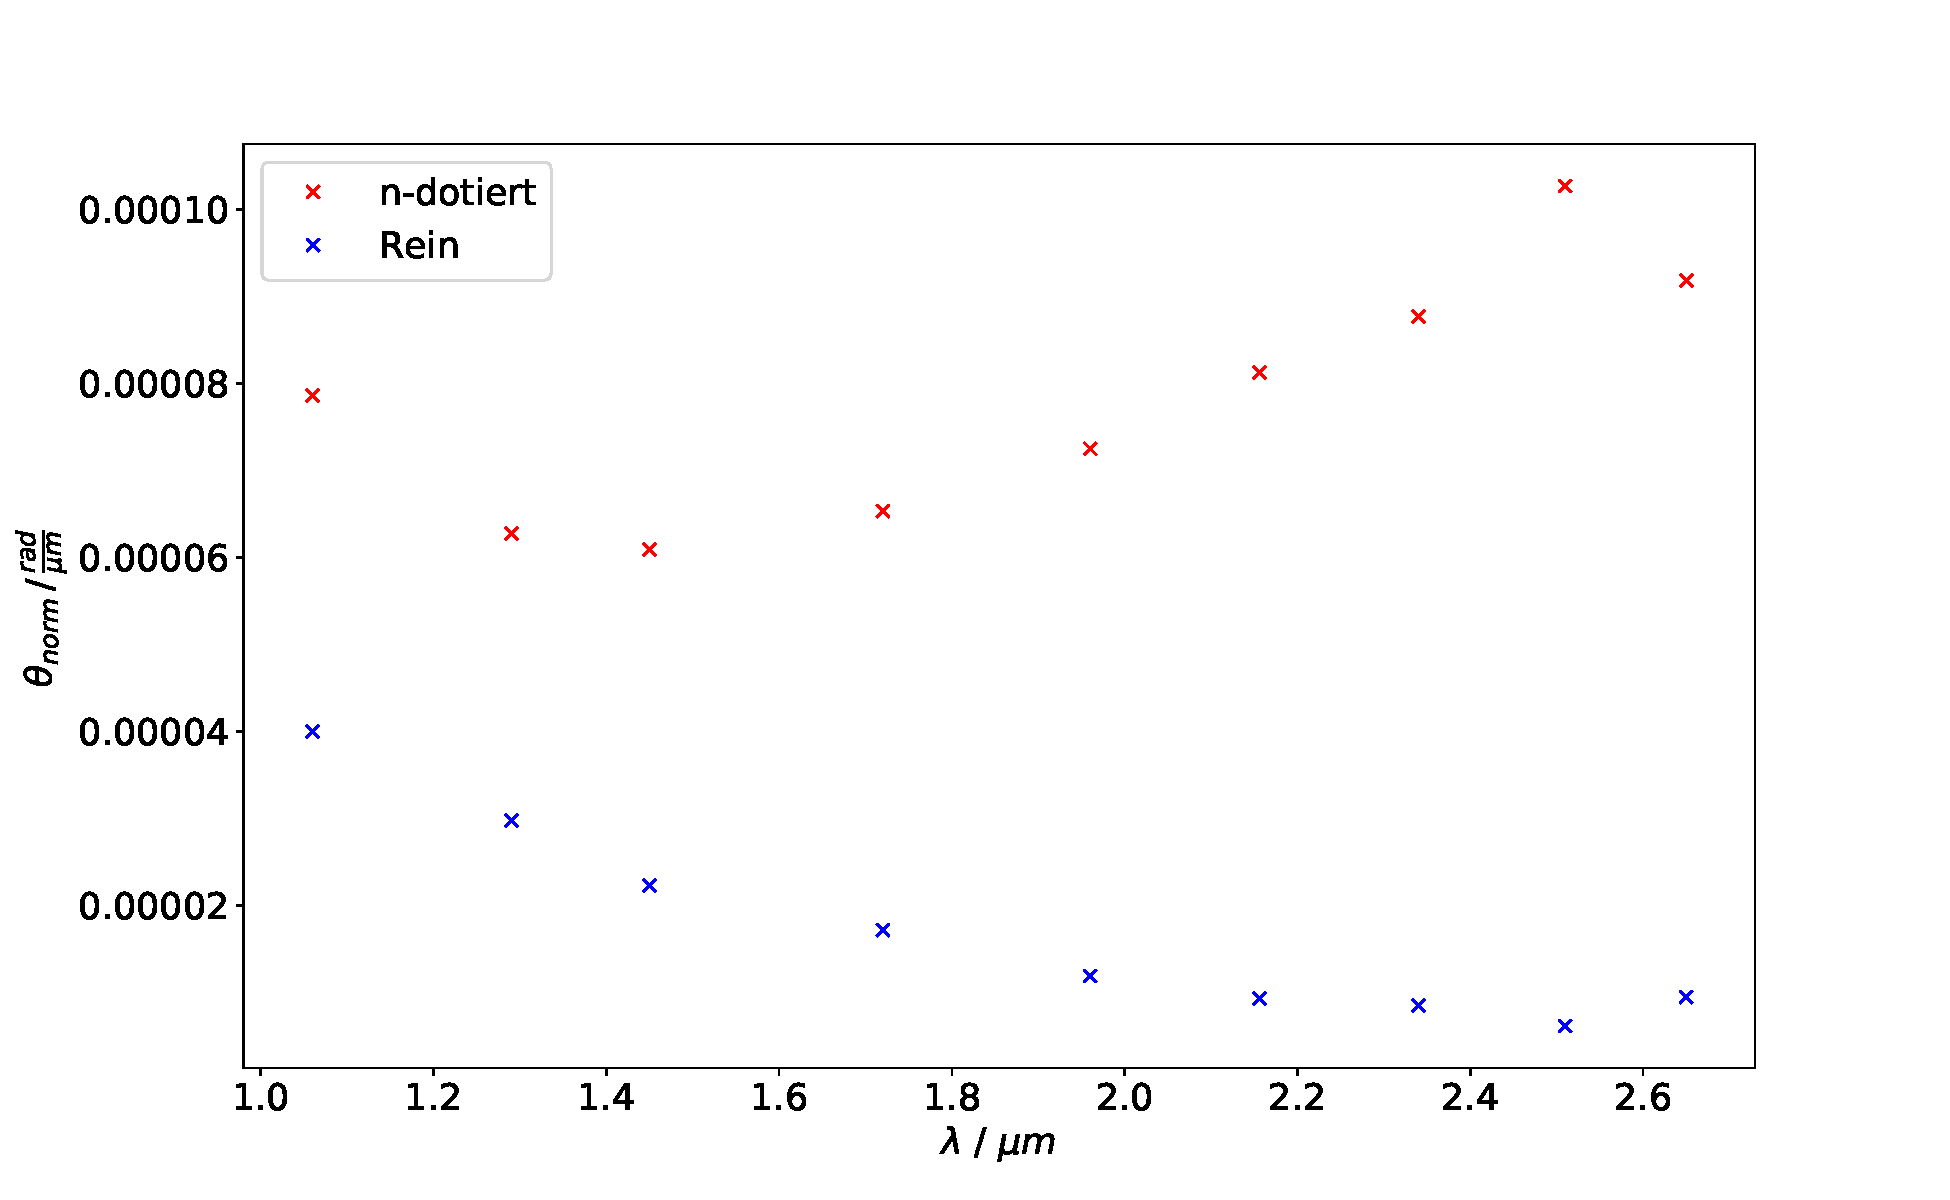
\includegraphics[width = \textwidth,keepaspectratio]{figure/Theta2_plot.pdf}
  \caption{Graphische Darstellung der normierten Drehwinkel, in Abhängigkeit der Wellenlänge, von der Probe 2 mit einer Dicke von $d=\SI{1296}{\micro\meter}$ und 
  der reinen Probe.}
  \label{fig:Drehwinkel_2}
\end{figure}
\FloatBarrier
Um die  Effektive Masse der Leitungselektronen bestimmen zu können, wird die Differenz der normierten Drehwinkel ermittelt
und gegen das Quadrat der Wellenlänge aufgetragen. Die Differenzen sind in Tabelle \ref{tab:Differenzen} aufgelistet.
\FloatBarrier
\begin{table}
  \centering
  \begin{tabular}{c c c}
    \toprule
    $\lambda^2$ / \SI{}{\square\micro\meter}&$\Delta_{\text{1}}$ / $\frac{\SI{}{\radian}}{\SI{}{\micro\meter}}$&$\Delta_{\text{2}}$ / $\frac{\SI{}{\radian}}{\SI{}{\micro\meter}}$\\
    \midrule 
    $\num{1.1}$&$\num{1.52e-4}$&$ \num{0.39e-4}$\\
    $\num{1.7}$&$\num{0.71e-4}$&$ \num{0.33e-4}$\\
    $\num{2.1}$&$\num{-0.02e-4}$&$\num{0.39e-4}$\\
    $\num{3.0}$&$\num{0.04e-4}$&$ \num{0.48e-4}$\\
    $\num{3.8}$&$\num{0.52e-4}$&$ \num{0.61e-4}$\\
    $\num{4.6}$&$\num{0.39e-4}$&$ \num{0.72e-4}$\\
    $\num{5.5}$&$\num{0.74e-4}$&$ \num{0.79e-4}$\\
    $\num{6.3}$&$\num{1.71e-4}$&$ \num{0.97e-4}$\\
    $\num{7.0}$&$\num{0.45e-4}$&$  \num{0.82e-4}$\\
    \bottomrule
  \end{tabular}
  \caption{Messwerte zur Bestimmung der effektiven Masse von Ladungselektronen.}
  \label{tab:Differenzen}
\end{table}
\FloatBarrier
Die Daten werden gegeneinander aufgetragen und die Funktion \eqref{eq:fit} wird an die Daten gefittet.
\begin{equation}
  \label{eq:fit}
  \theta_{\text{frei}} = f(\lambda^2) = a\cdot \lambda^2
\end{equation}
Die Daten aus Tabelle \ref{tab:Differenzen} und der dazugehörige Fit sind in den Abbildungen \ref{fig:fit1} und \ref{fig:fit2} 
dargestellt.
\FloatBarrier
\begin{figure}
  \centering
  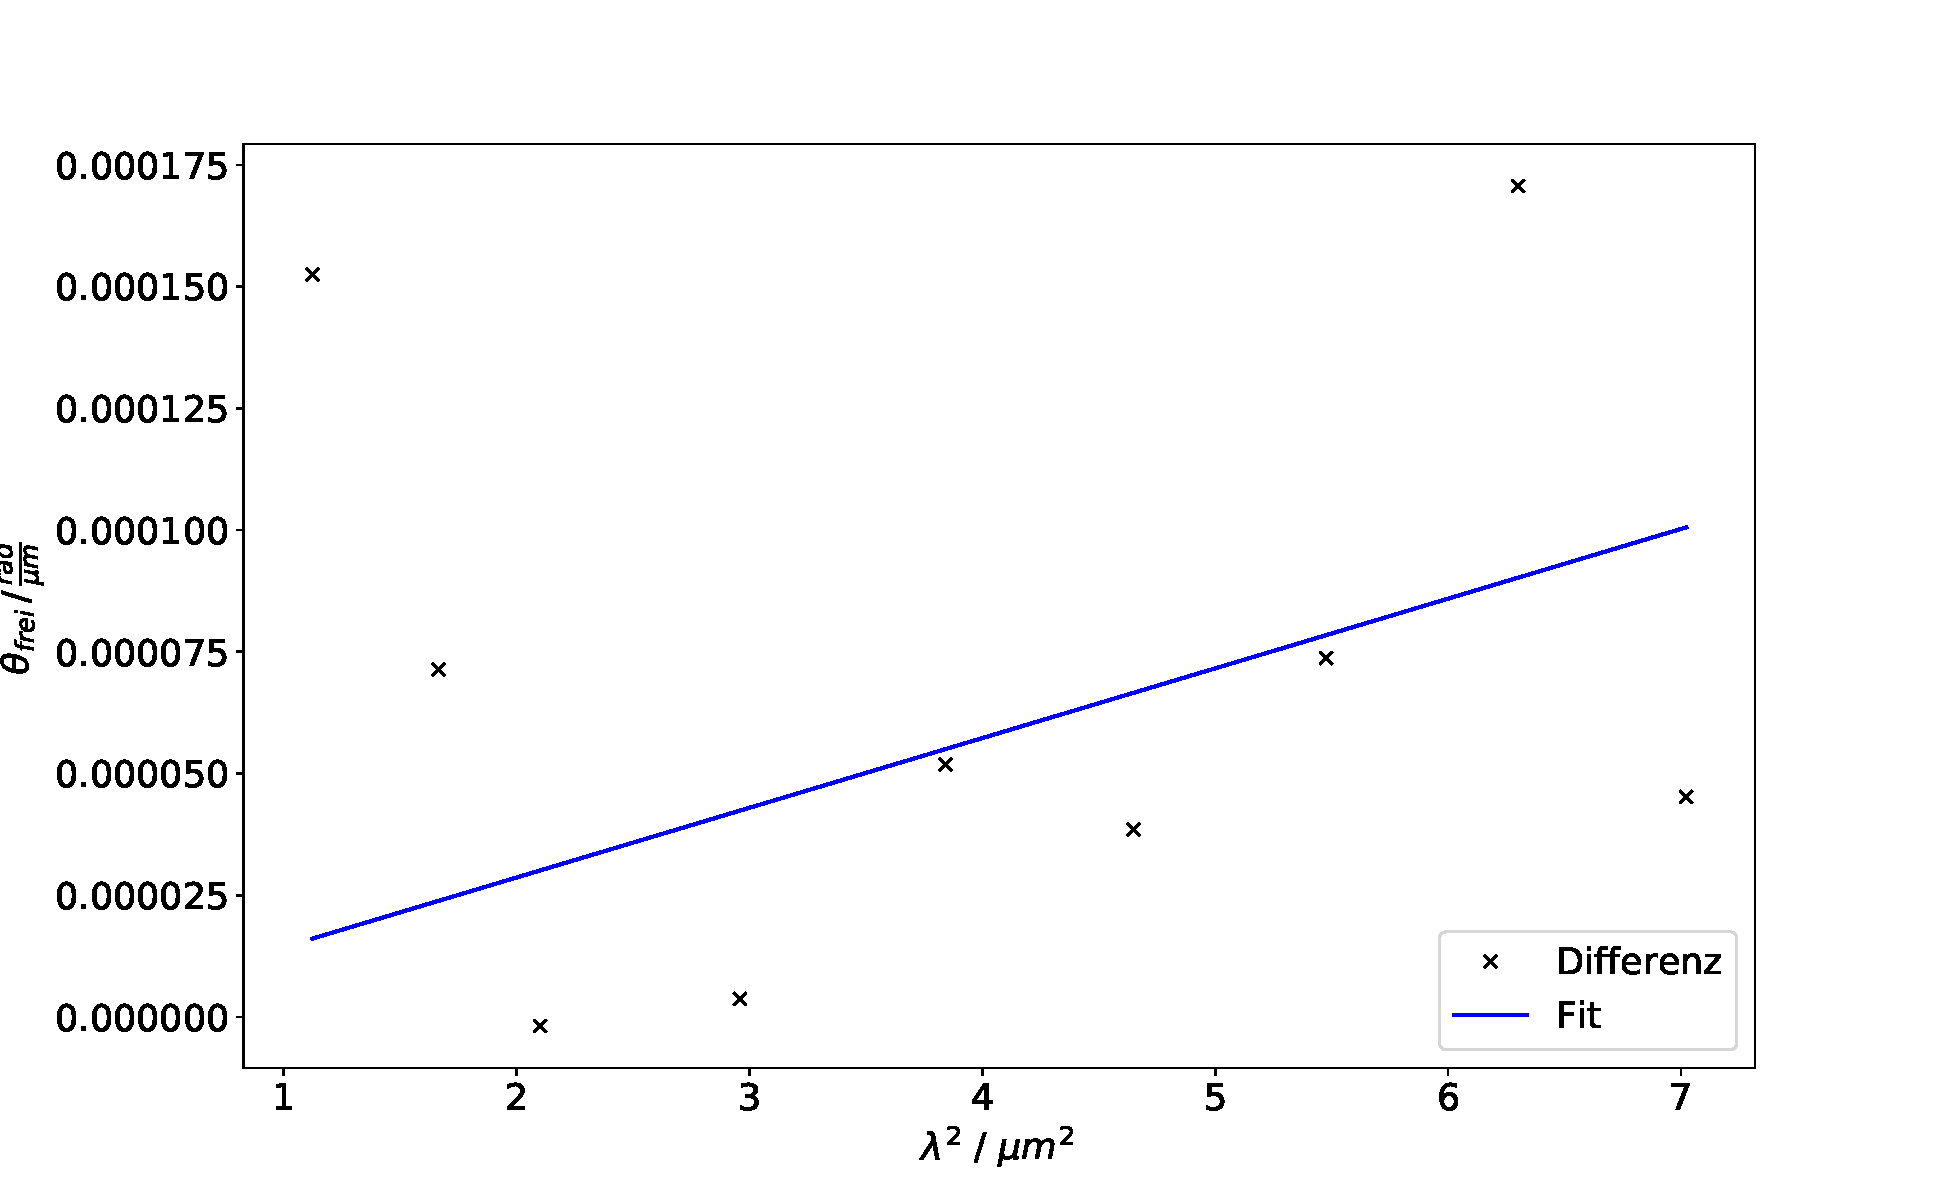
\includegraphics[width = \textwidth]{figure/Theta1_diff_plot.pdf}
  \caption{Plot zur Bestimmung der effektiven Masse mittels Probe 1}
  \label{fig:fit1}
\end{figure}
\begin{figure}
  \centering
  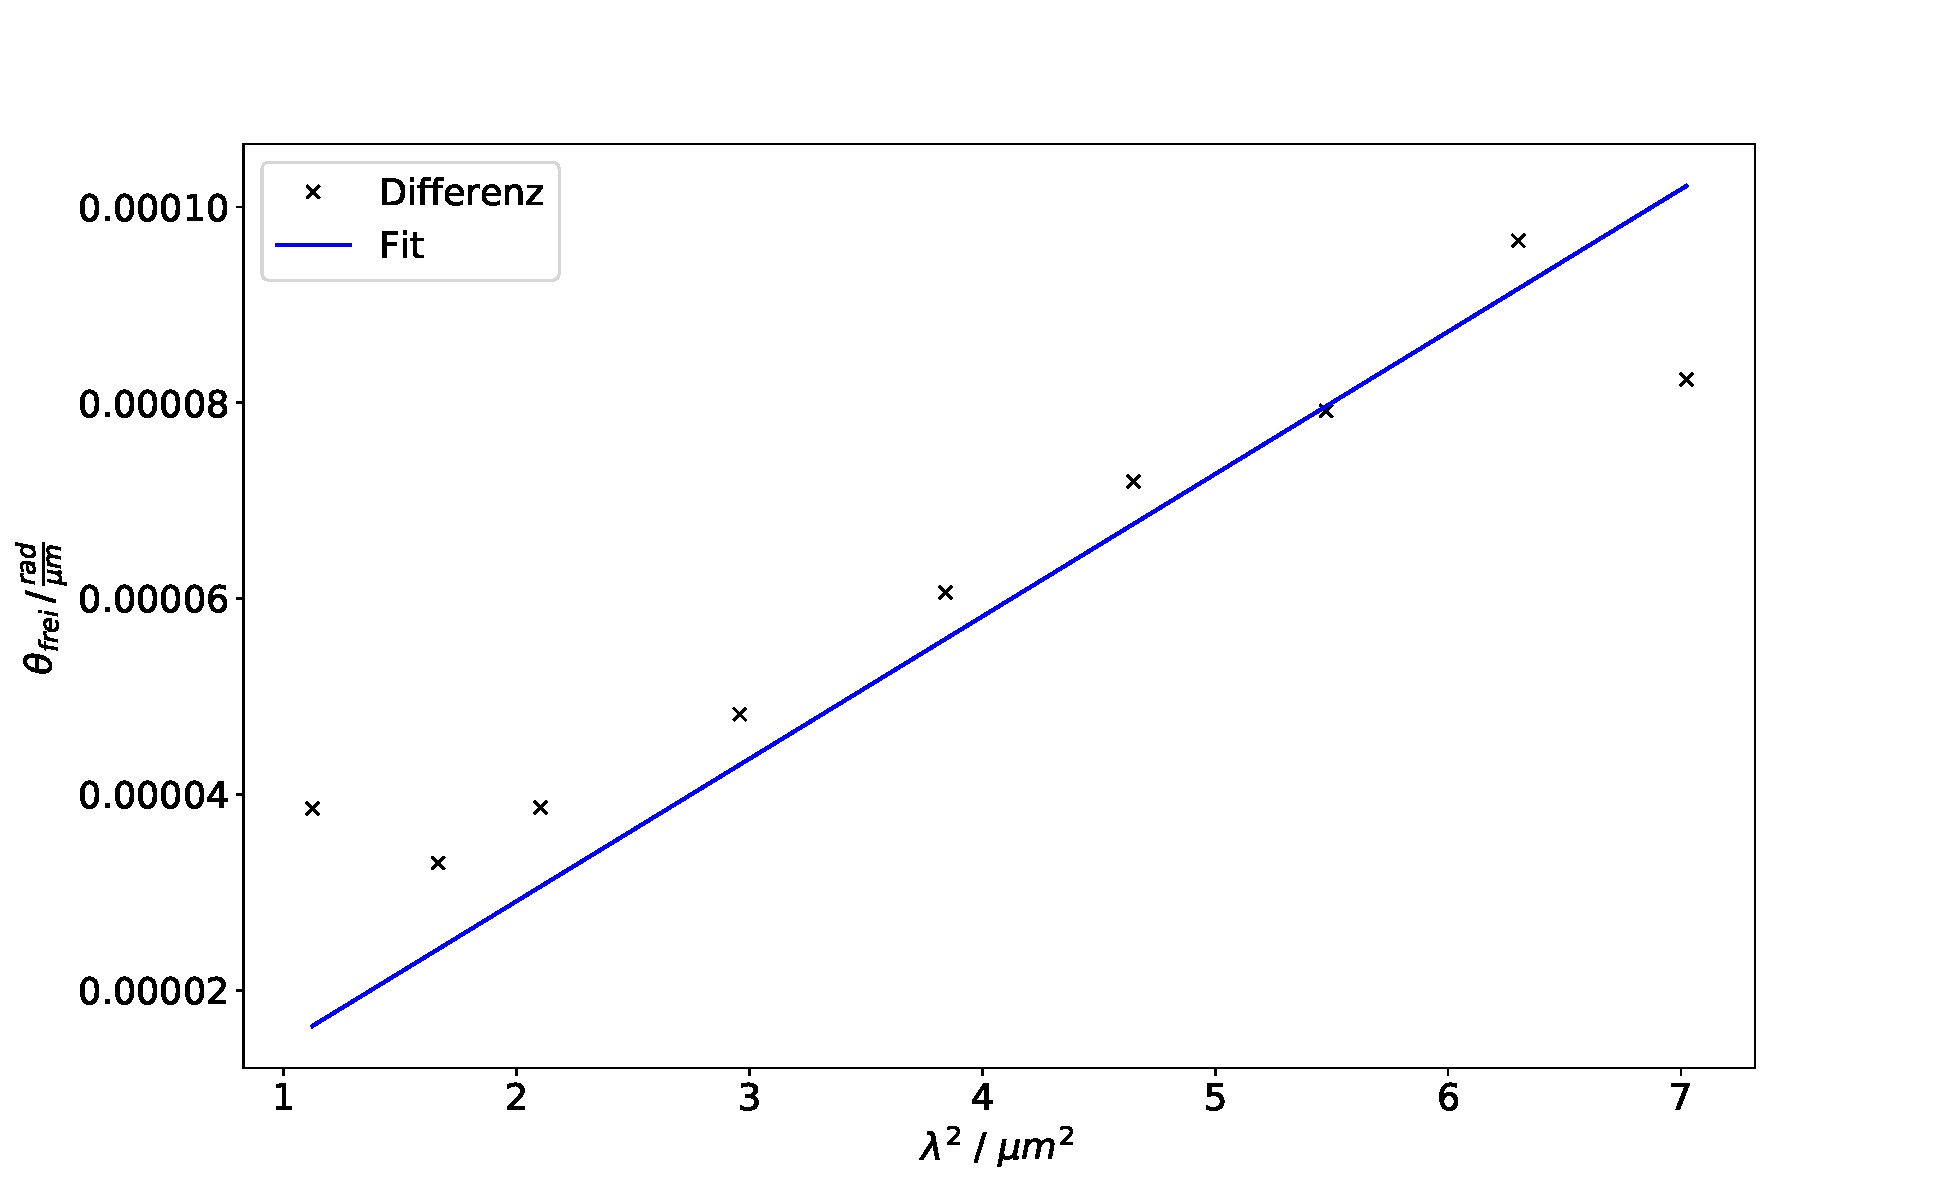
\includegraphics[width = \textwidth]{figure/Theta2_diff_plot.pdf}
  \caption{Plot zur Bestimmung der effektiven Masse mittels Probe 2}
  \label{fig:fit2}
\end{figure}
\FloatBarrier
Die Fitparameter der beiden Funktionen sind:
\begin{align*}
  a_{\text{1}} =& \num{3(1)e13}  \,\frac{\SI{}{\radian}}{\SI{}{\cubic\meter}}\\
  a_{\text{2}} =& \num{2.9(1)e13}\,\frac{\SI{}{\radian}}{\SI{}{\cubic\meter}}.
\end{align*}
Der Wert $a$ kann in die folgende Gleichung eingesetzt werden, um die effektive Masse zu bestimmen.
\begin{align*}
  &\theta_{\text{frei}} = \frac{\symup{e}_0^3}{8\pi^2\epsilon_0\symup{c}^3 \left(m^*\right)^2}\lambda^2\frac{NB}{n}\\
  &\implies \left(m^*\right)=\sqrt{\frac{\symup{e}_0^3}{8\pi^2\epsilon_0\symup{c}^3} \left(\frac{\lambda^2}{\theta_{\text{frei}}}\right)\frac{NB}{n} }\\
  &\implies \left(m^*\right)=\sqrt{\frac{\symup{e}_0^3}{8\pi^2\epsilon_0\symup{c}^3} \left(\frac{1}{a}\right)\frac{NB}{n} }
\end{align*}
Der Brechungsindex von Gallium-Arsenide ist Abhängigkeit von der Wellenlänge, allerdings ist der Brechungsindex ab 
einer Wellenlänge von $\lambda=\SI{1000}{\nano\meter}$ nahezu konstant \cite{Brechungsindex}. Daher wird 
für die Berechnung der effektiven Masse der Wert $n=\num{3.35}$ verwendet.
Die effektive Masse beträgt:
\begin{equation*}
  m^*_1 = \SI{4.7(8)e-32}{\kilo\gram}\qquad m^*_2 = \SI{7.1(2)e-32}{\kilo\gram}
\end{equation*}
\begin{equation*}
  m^*_{\text{mittel}}=\SI{6(1)e-32}{\kilo\gram}
\end{equation*}